\section{High energy physics applications}
\label{sec:hep}

\subsection{B physics}

\subsubsection{Data sample}

In order to demonstrate the functionality of the toolkit, data samples generated
from the RapidSim package~\cite{rapid} are used. The interesting signal is chosen
to be the $\Bs\to\jpsi(\to\mu\mu )\phi (\to\PK\PK )$ decay, and the background is
the $\Dz\to\pi\pi\pi\pi$ decay. A total of 10000 candidates is generated for each decay.

\subsubsection{Training of the original classifier}
\label{sec:orig_training}

The machine learning classifier, using the Keras framework~\cite{keras,adam},
is constructed as a locally connected first layer (in which filters are applied
to different regions in contrast to a full convolution layer), followed by a pooling layer,
and a standard dense layer. The exact definition can be found below.
\begin{lstlisting}
classifier = Sequential()
classifier.add(LocallyConnected1D(
filters = 90, kernel_size = 2,
activation = 'sigmoid',
input_shape = (len(setTrain[0]), 1)))
classifier.add(GlobalMaxPooling1D())
classifier.add(Dense(30, activation = 'sigmoid'))
classifier.add(Dense(1, activation = 'sigmoid'))
classifier.compile(optimizer = 'adam',
loss = 'binary_crossentropy'
, metrics = ['accuracy'])
\end{lstlisting}

The neural network is trained using kinematic properties of the respective decays.
These include the pseudorapidity, $\eta$, and momentum transverse to the direction of the
input proton beams, \pt, of the decaying particle. In addition, the minimum and maximum \pt and $\eta$
of the final state particles is used. The signal and background distributions of the input variables
are shown in Fig.~\ref{fig:inputs}.
%
\begin{figure*}[t]
\centering
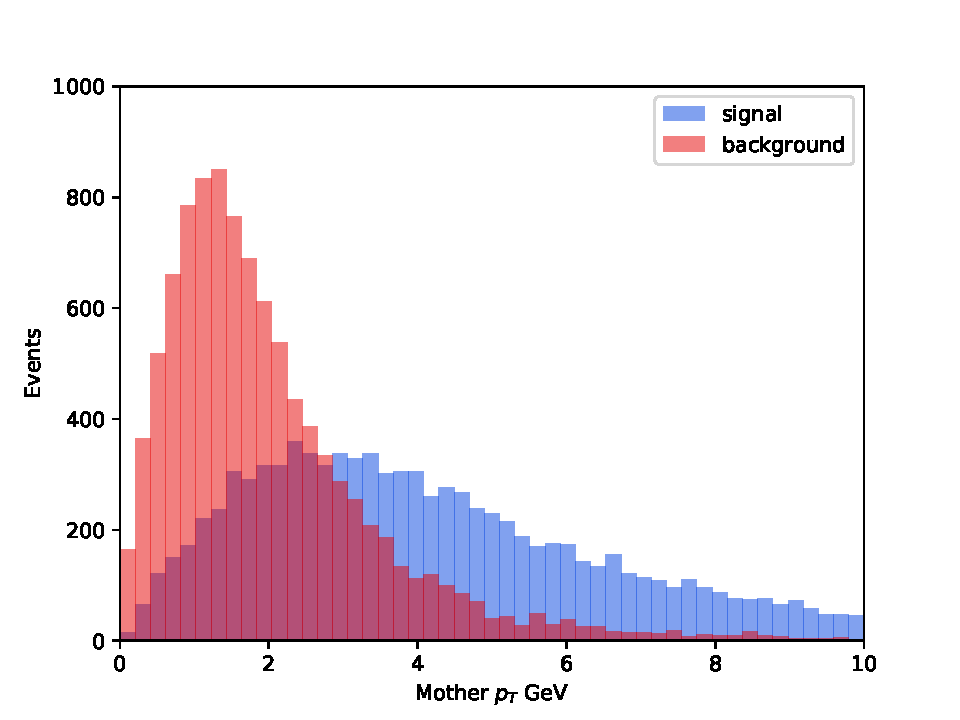
\includegraphics[width=0.33\textwidth]{pt_comp}
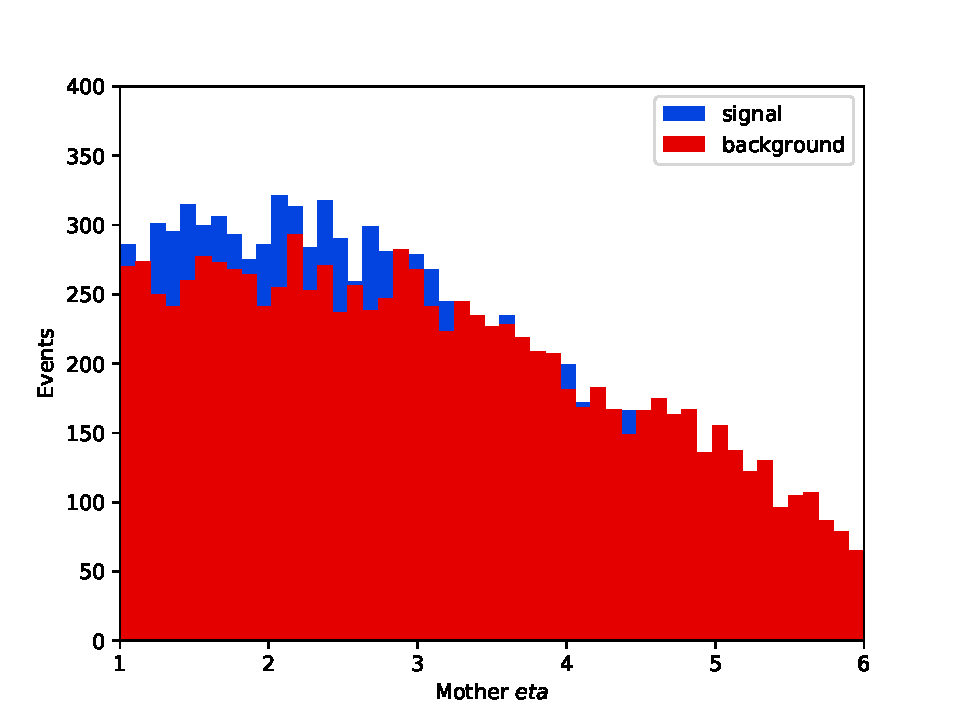
\includegraphics[width=0.33\textwidth]{eta_comp}
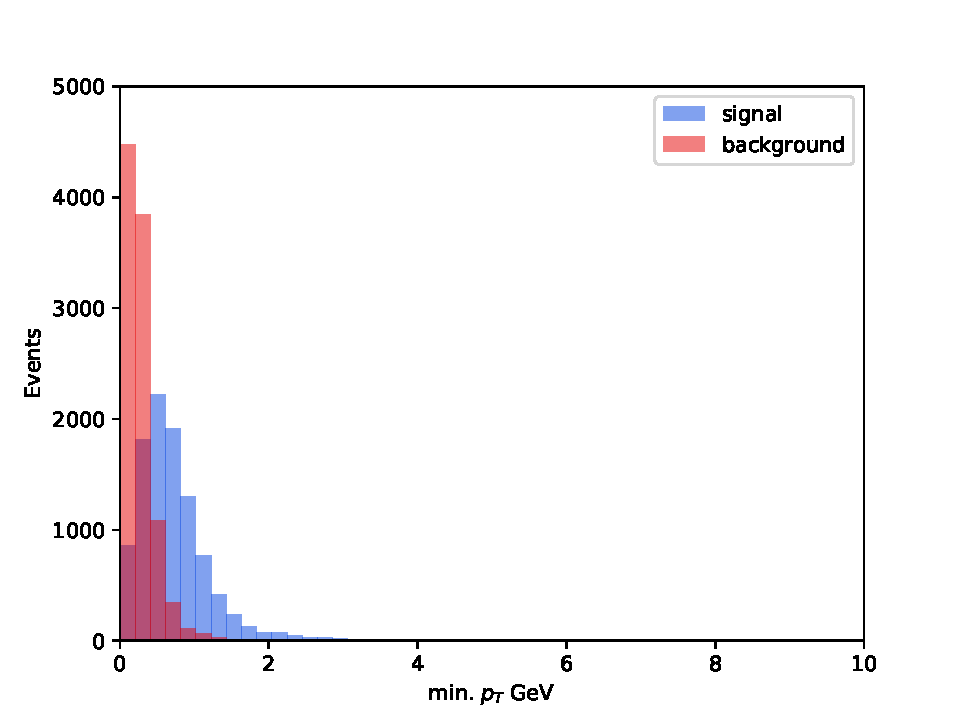
\includegraphics[width=0.33\textwidth]{minpt_comp}
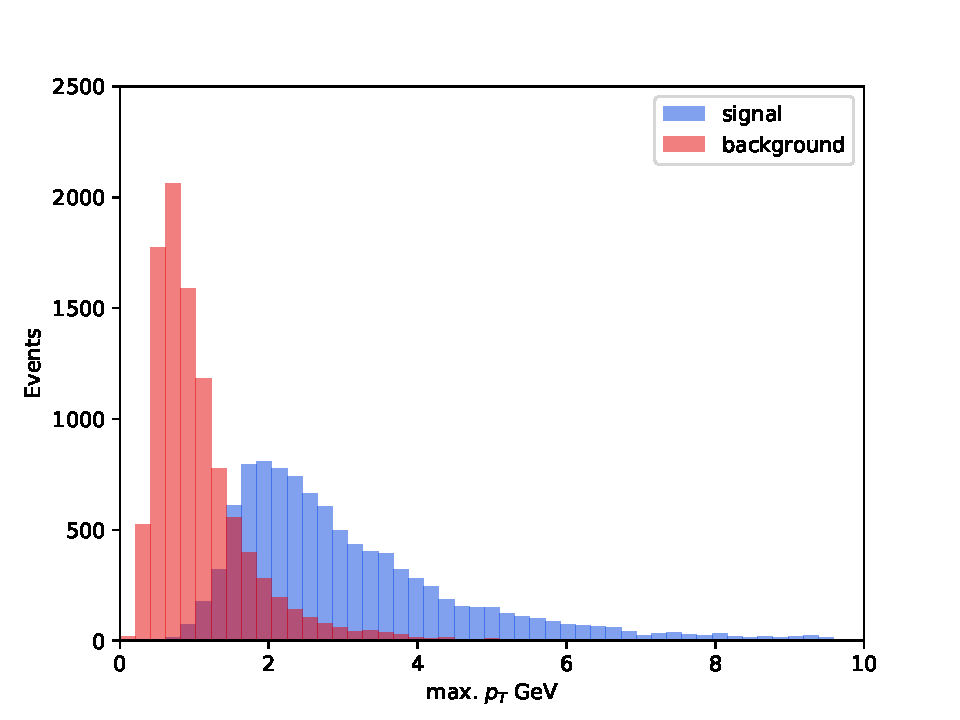
\includegraphics[width=0.33\textwidth]{maxpt_comp}
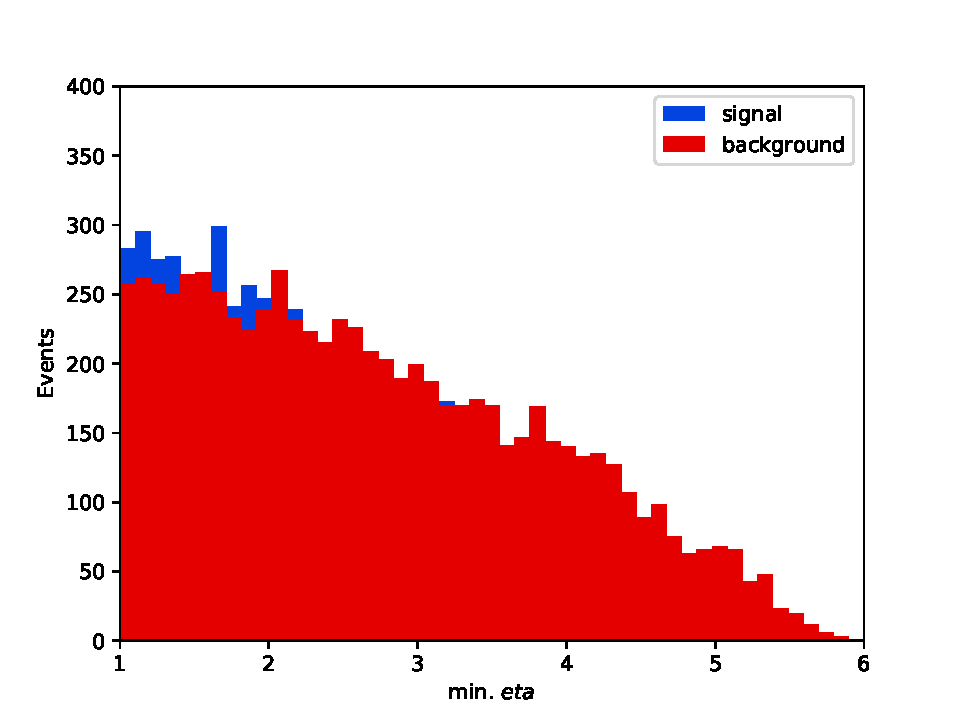
\includegraphics[width=0.33\textwidth]{mineta_comp}
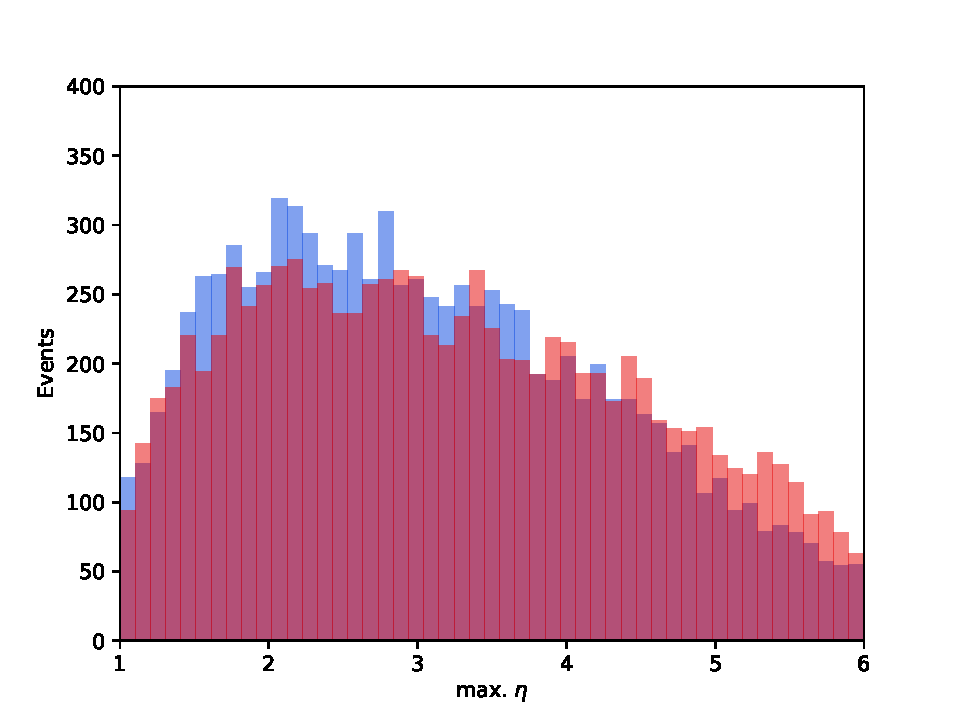
\includegraphics[width=0.33\textwidth]{maxeta_comp}
\caption{\small Comparison of the signal and background distributions
used to train the Keras B decay classifier.}
\label{fig:inputs}
\end{figure*}

In the training of the original classifier, half of the data is
reserved in order to test for overtraining.
%The output probability distributions of the signal and background samples
%after the training are shown in Fig.~\ref{fig:output}.
%It can be seen that the test and training samples are in good agreement,
%showing that the original SciKit-Learn classifier is not significantly overtrained.
%\begin{figure*}[t]
%\centering
%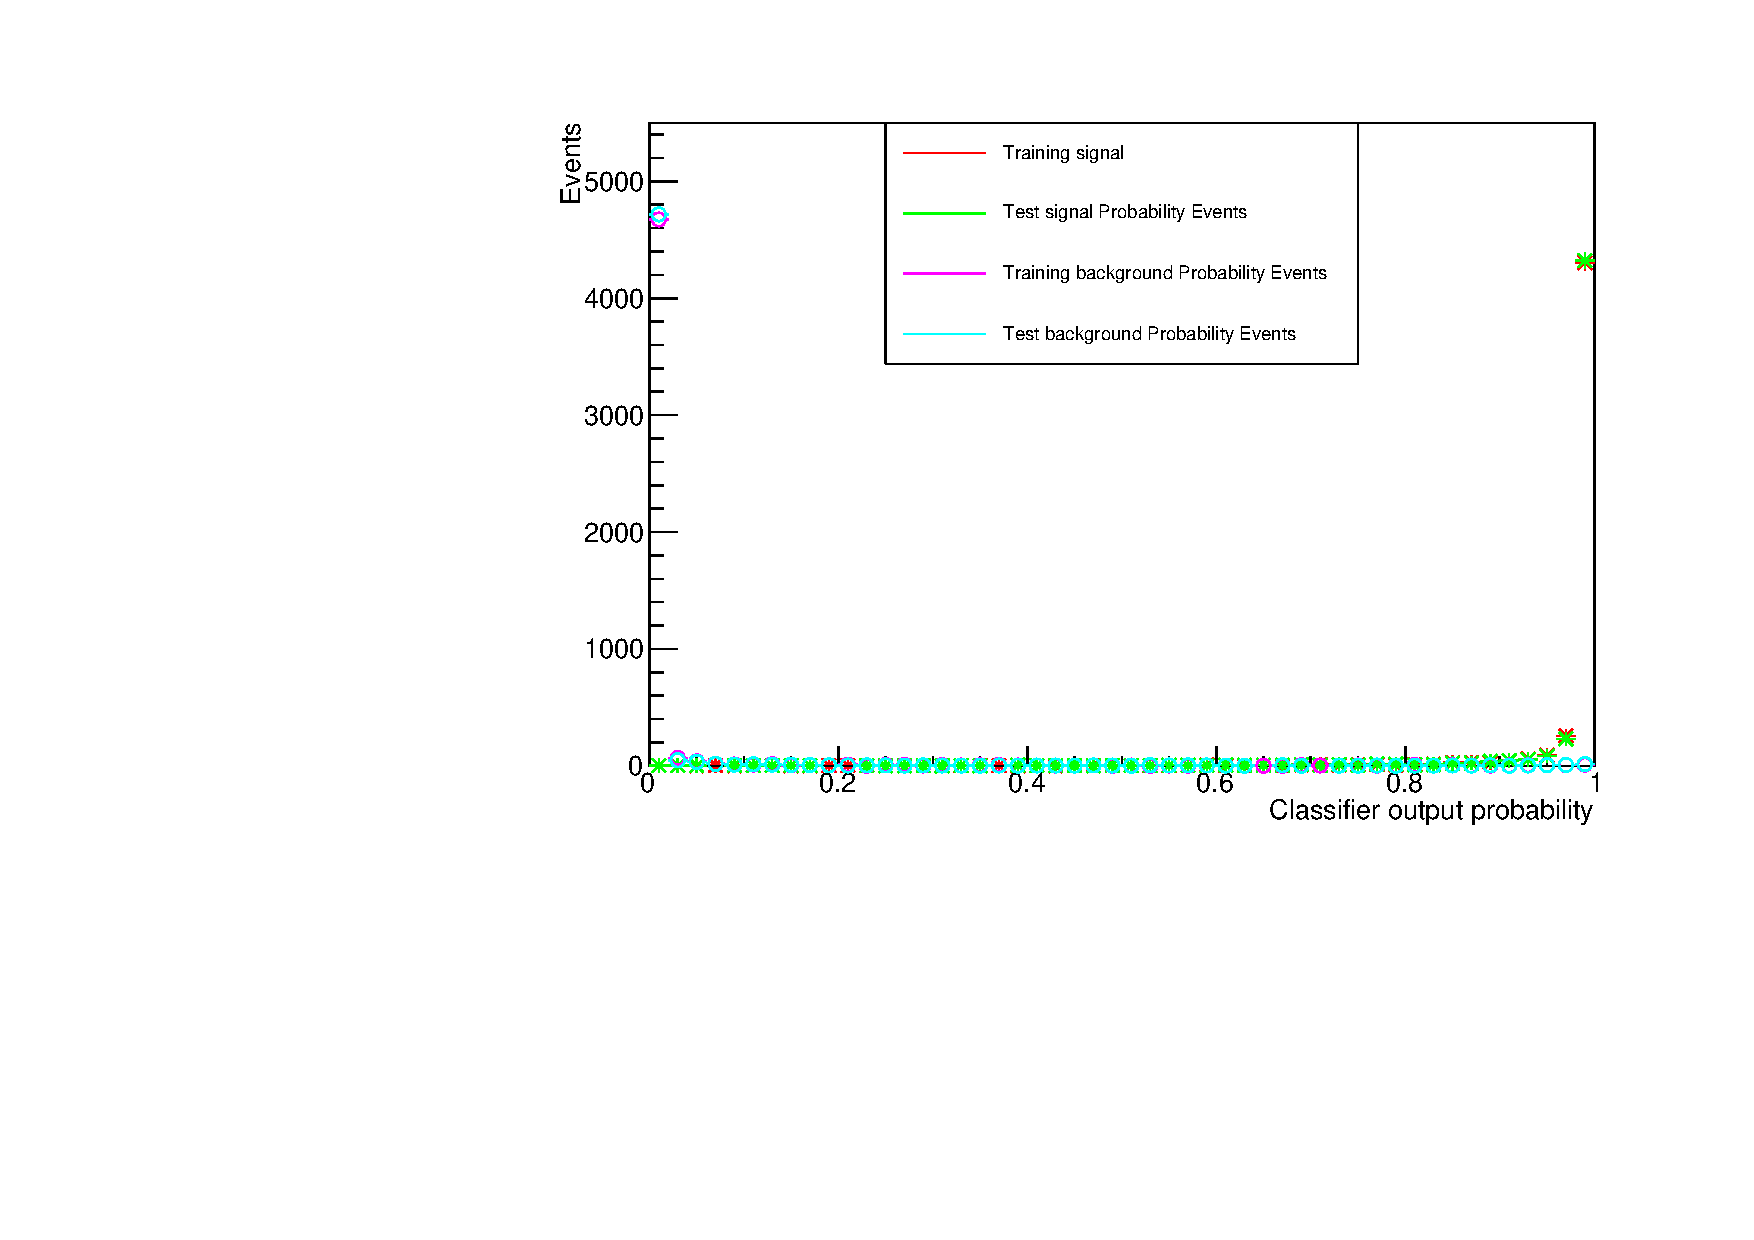
\includegraphics[width=0.45\textwidth]{event_probability}
%\caption{\small
%Output distributions of the signal and background training and
%test samples from the classifier after training.
%}
%\label{fig:output}
%\end{figure*}


\subsection{Jet separation}
\label{sec:hepGPD}

\subsubsection{Data sample}

A further demonstration is provided demonstrating a classifiers ability to separate different
kinds of jets. The data sample to show this has been generated from Pythia~\cite{Sjostrand:2007gs}
simulating pp collisions at 14\tev.
The jets themselves are reconstructed in the Rivet analysis framework~\cite{Buckley:2010ar}
and are created using the FastJet~\cite{Cacciari:2011ma} package using the $K_t$ algorithm~\cite{Salam:2007xv}
(the definition
of the $K_t$ variable and a review of jet reconstruction algorithms
may be found in Refs~\cite{kt} and \cite{Atkin:2015msa} respectively).
A jet \pt requirement of 20\gev is imposed on all jets.
All other parameters remain at the default values for Rivet version 2.5.4.
The signal sample is chosen to correspond to a $qg\to Wq$ type of interaction,
whereas the background is chosen to correspond to a $gg \to gg$ type. These correspond
to the Rivet analyses named {\tt MC\_WJETS} and {\tt MC\_QCD}, respectively.
Jets that originate from gluons in the final state form a background to many
analyses, therefore efficient rejection of such processes is important in making
measurements~\cite{Komiske:2016rsd}.

\subsubsection{Training of the original classifier}

The machine learning classifier chosen is also a Keras-based convolutional neural net,
constructed in an similar way as described in Sec~\ref{sec:orig_training}
\begin{lstlisting}
classifier = Sequential()
classifier.add(LocallyConnected1D(
filters = 90, kernel_size = 2,
activation = 'sigmoid',
input_shape = (len(setTrain[0]), 1)))
classifier.add(GlobalMaxPooling1D())
classifier.add(Dense(30, activation = 'sigmoid'))
classifier.add(Dense(1, activation = 'sigmoid'))
classifier.compile(optimizer = 'adam',
loss = 'binary_crossentropy'
, metrics = ['accuracy'])
\end{lstlisting}

The training data is based around the properties of the measured jets. The list of features
taken consists of the azimuthal angle, $\phi$, $\eta$ of the jet; the spread of neutral and 
hadronic contributions to the jet in the $\phi$, $\eta$ variables, along with average and energy weighted
kinematic variables. In total 17 different features are used.
The signal and background distributions of the input variables
are shown in Fig.~\ref{fig:inputsGPD}.
%
\begin{figure*}[t]
\centering
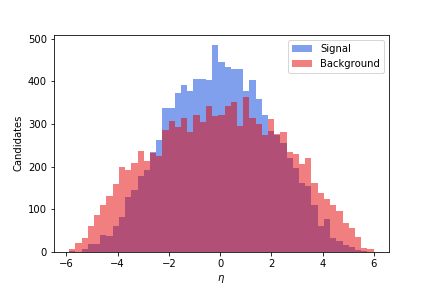
\includegraphics[width=0.33\textwidth]{gpd_inputs/input_gpd_eta}
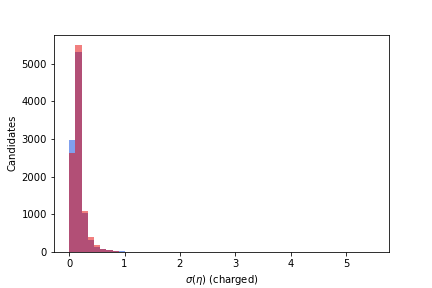
\includegraphics[width=0.33\textwidth]{gpd_inputs/input_gpd_eta_spread_charged}
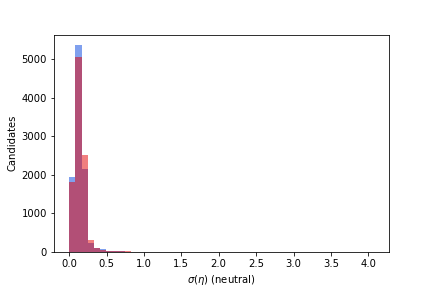
\includegraphics[width=0.33\textwidth]{gpd_inputs/input_gpd_eta_spread_neutral}
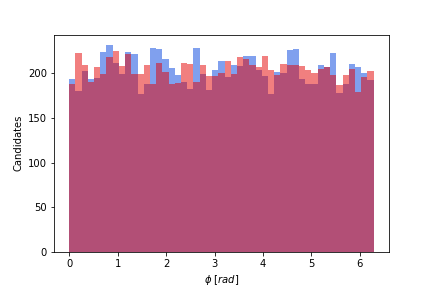
\includegraphics[width=0.33\textwidth]{gpd_inputs/input_gpd_phi}
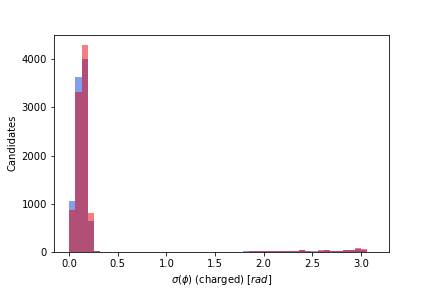
\includegraphics[width=0.33\textwidth]{gpd_inputs/input_gpd_phi_spread_charged}
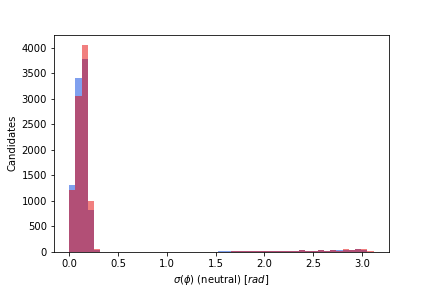
\includegraphics[width=0.33\textwidth]{gpd_inputs/input_gpd_phi_spread_neutral}
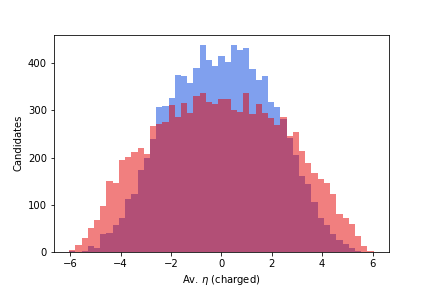
\includegraphics[width=0.33\textwidth]{gpd_inputs/input_gpd_hAvEta}
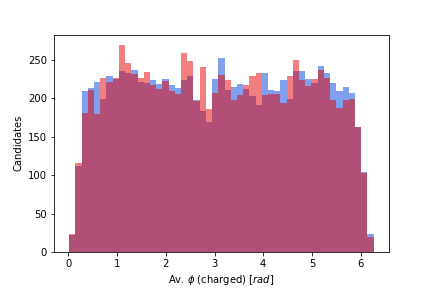
\includegraphics[width=0.33\textwidth]{gpd_inputs/input_gpd_hAvPhi}
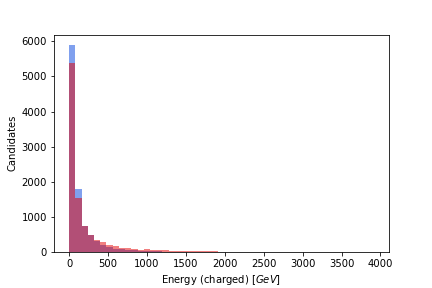
\includegraphics[width=0.33\textwidth]{gpd_inputs/input_gpd_hEnergy}
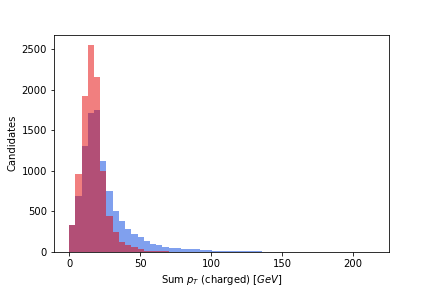
\includegraphics[width=0.33\textwidth]{gpd_inputs/input_gpd_hSumPT}
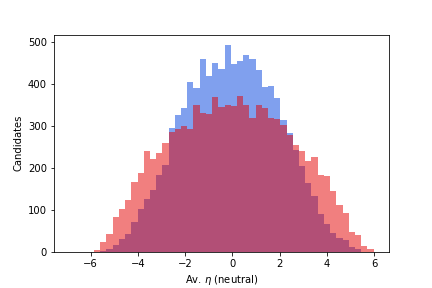
\includegraphics[width=0.33\textwidth]{gpd_inputs/input_gpd_nAvEta}
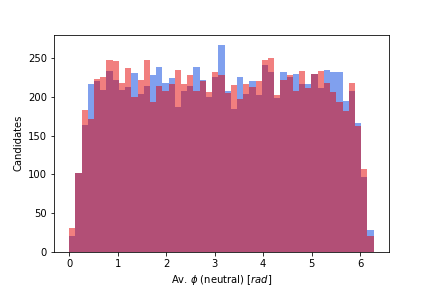
\includegraphics[width=0.33\textwidth]{gpd_inputs/input_gpd_nAvPhi}
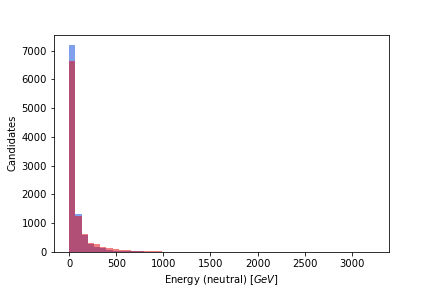
\includegraphics[width=0.33\textwidth]{gpd_inputs/input_gpd_nEnergy}
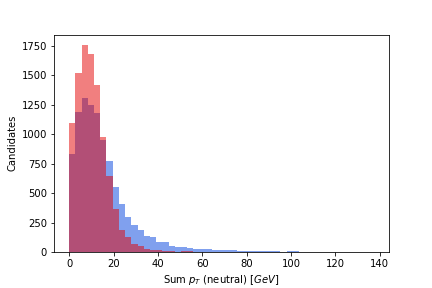
\includegraphics[width=0.33\textwidth]{gpd_inputs/input_gpd_nSumPT}
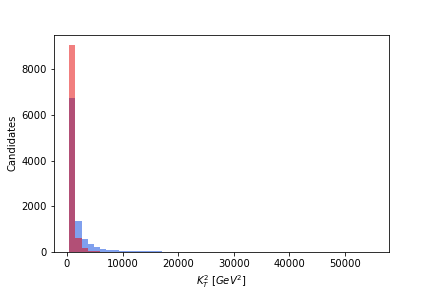
\includegraphics[width=0.33\textwidth]{gpd_inputs/input_gpd_kt2}
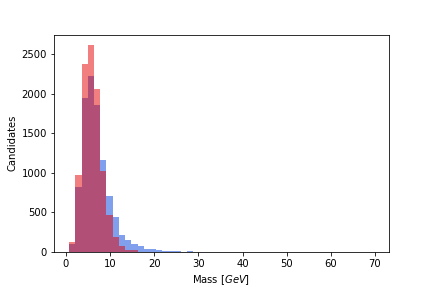
\includegraphics[width=0.33\textwidth]{gpd_inputs/input_gpd_mass}
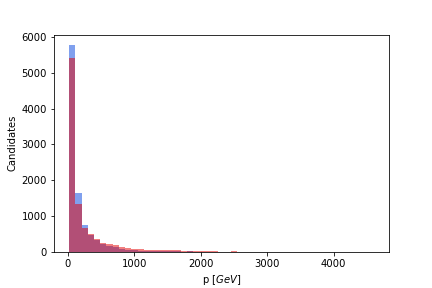
\includegraphics[width=0.33\textwidth]{gpd_inputs/input_gpd_mom}
\caption{\small Comparison of the signal and background distributions
used to train the Keras jet separation classifier.}
\label{fig:inputsGPD}
\end{figure*}

\subsection{Drone conversions}

The drone neural networks are trained following the procedure outlined in Sec.~\ref{sec:dlearn},
In total, 300 epochs are used with
the learning rate of the stochastic gradient descent set to 0.05.
The value of $\kappa$ is chosen to be 0.02, the value of $b$ is chosen to
be 0.04 and the value of $m$ is chosen to be 50.

The loss history of the drone approximations are shown in Fig.~\ref{fig:loss}
as a function of epoch number.
The convergence is also shown in Fig.~\ref{fig:iterdiff}, which shows
the difference in the value of the loss function with respect to the previous
epoch. The epochs that trigger an increase in the number of hyperparameters
are also overlaid.
In total for the case of B decays and for the case of the jet separation classifier, 
an increase was triggered 10 times.
The total number
of parameters in the final drone neural networks are therefore 121 and 286 for the B decay drone
and the jet separation drone, respectively. It is interesting
to note that with the algorithm design of Sec.~\ref{sec:dlearn}, the introduction
of the new parameter space causes the drone networks to learn faster, as evidenced by
increases in Fig.~\ref{fig:iterdiff} with continuing descent of the loss functions.
%
The performance of the original classifiers compared to the drone classifiers are shown in Figure~\ref{fig:roc}.
\begin{figure*}[t]
\centering
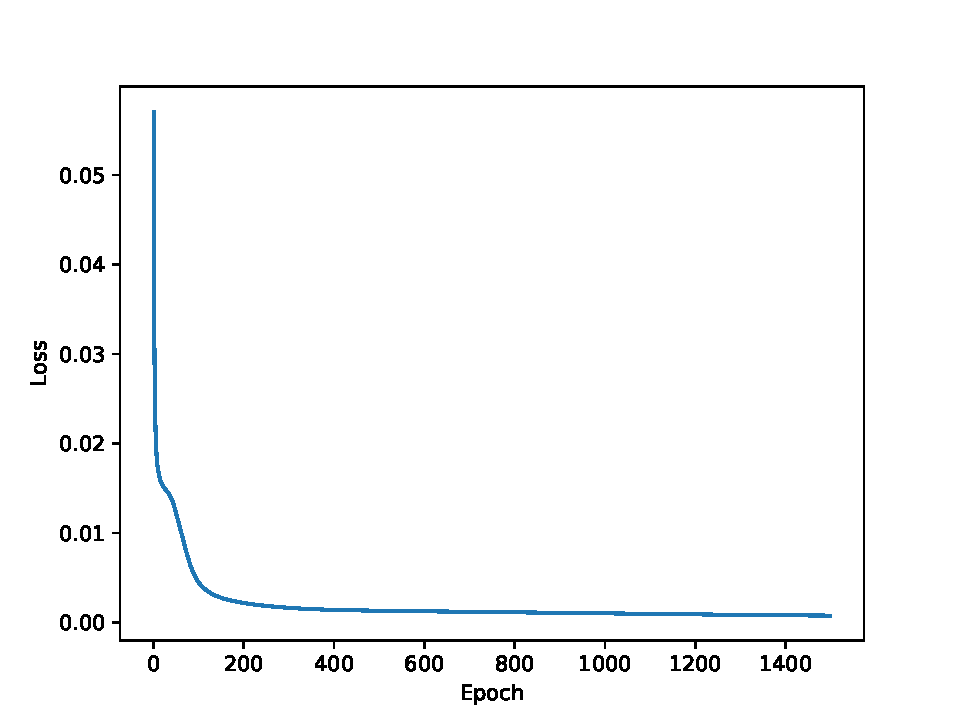
\includegraphics[width=0.45\textwidth]{loss_history}
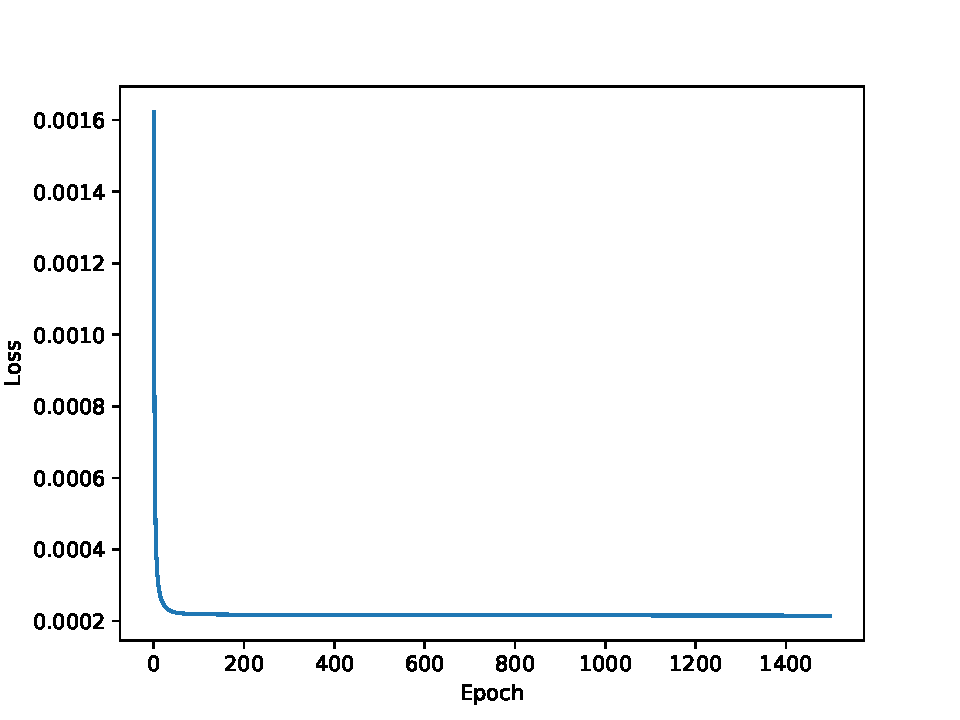
\includegraphics[width=0.45\textwidth]{loss_history_gpd}
\caption{\small
Convergence of the loss function during the drone training
  for the case of the B
  decay (left) and jet separation (right) examples.
}
\label{fig:loss}
\end{figure*}
\begin{figure*}[t]
\centering
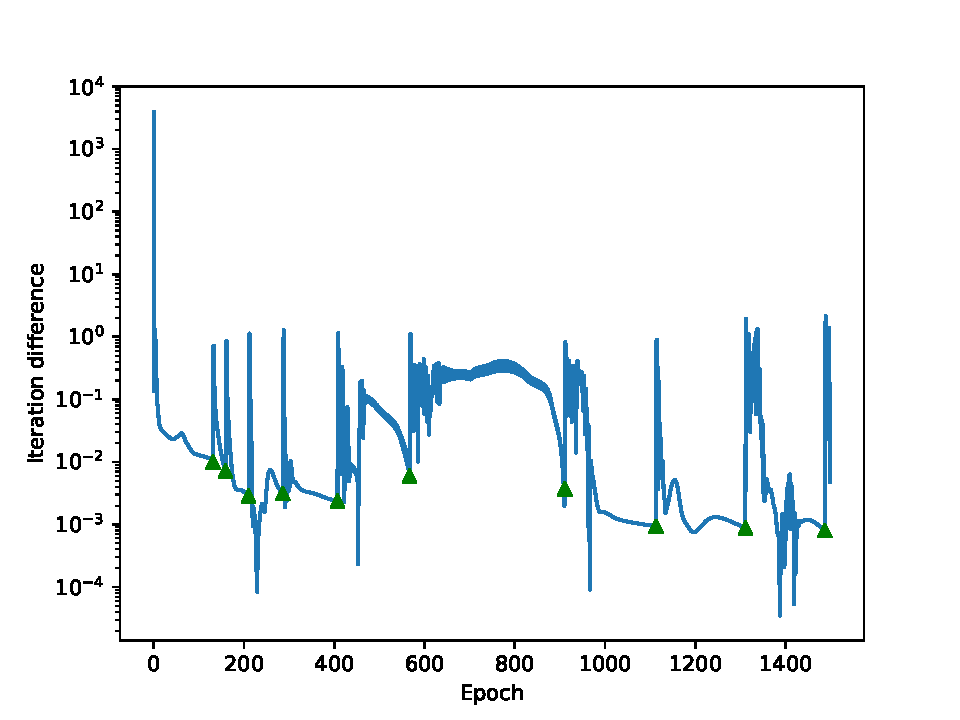
\includegraphics[width=0.45\textwidth]{diff_history}
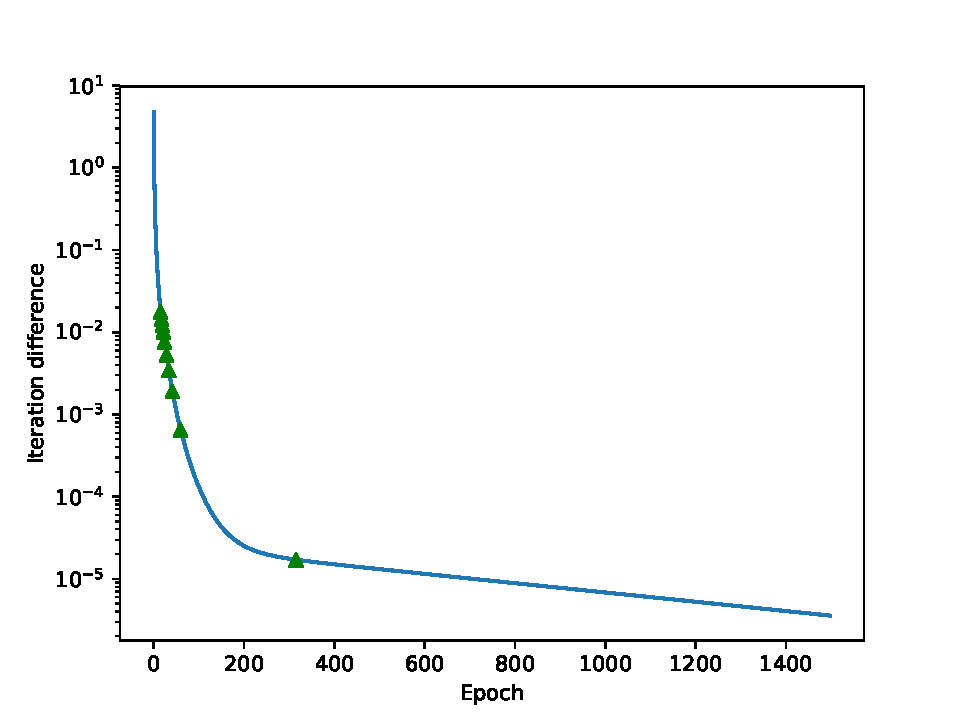
\includegraphics[width=0.45\textwidth]{diff_history_gpd}
\caption{\small
Difference in the loss function with respect to the previous iteration
  for the case of the B
  decay (left) and jet separation (right) examples.
  The green triangles
depict the epoch number in which the number of hyperperameters was increased.
}
\label{fig:iterdiff}
\end{figure*}
\begin{figure*}[t]
\centering
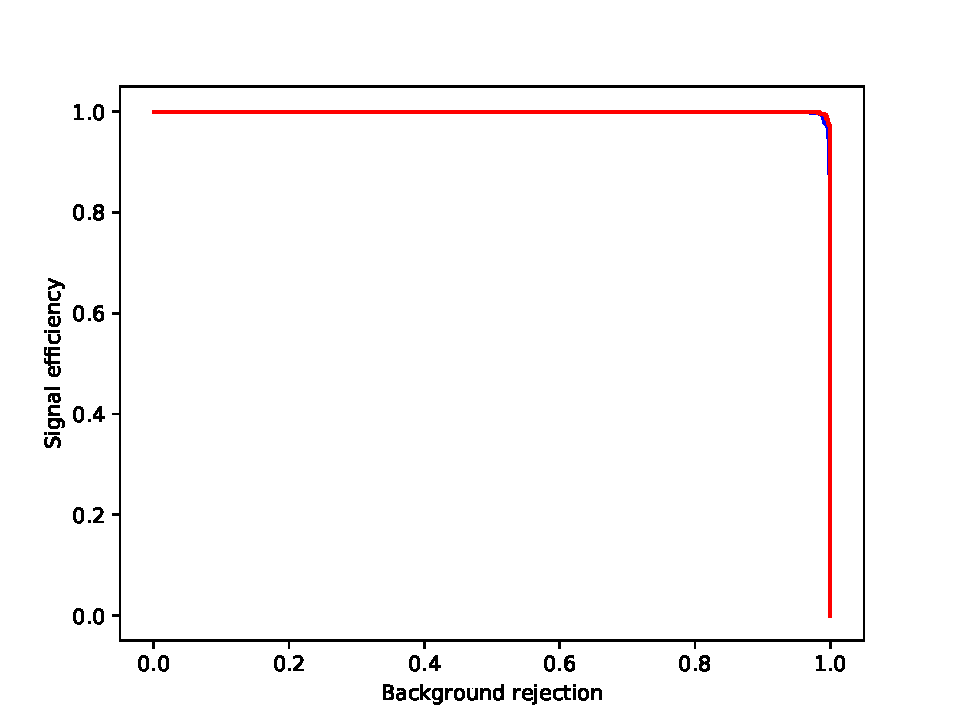
\includegraphics[width=0.45\textwidth]{roc}
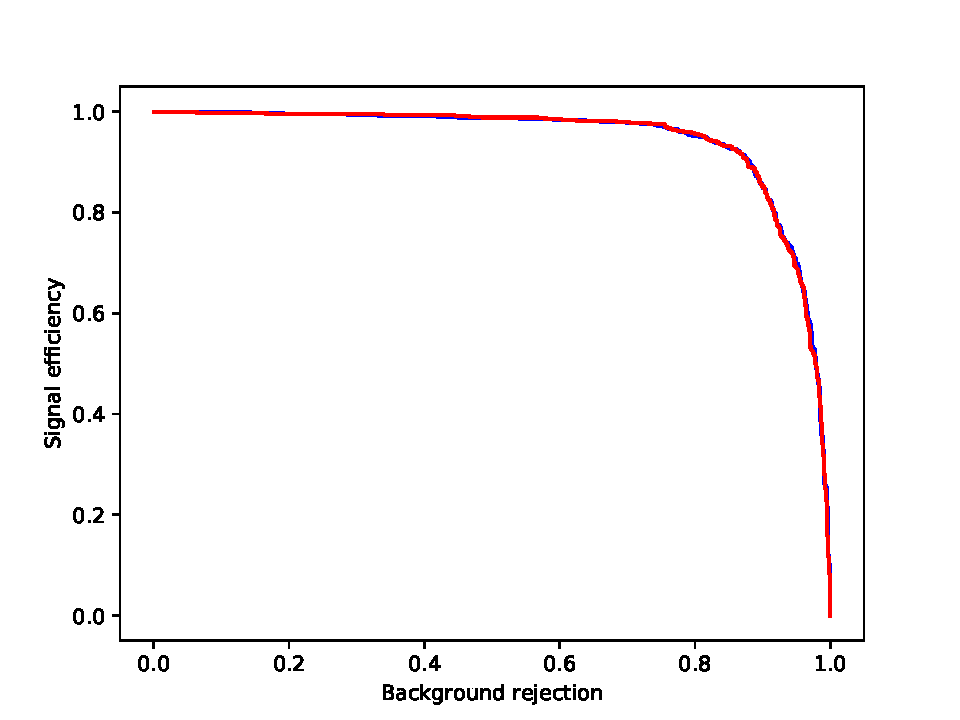
\includegraphics[width=0.45\textwidth]{roc_gpd}
\caption{\small
  Signal efficiency versus background rejection of the original classifier (red) and drone
  approximation (blue)
  for the case of the B
  decay (left) and jet separation (right) examples.
}
\label{fig:roc}
\end{figure*}


\section{Drone storage and transferability and suitability
for low-latency environments}
\label{sec:storage}

The hyperparameters and structure of the drone are required to be
portable and easily stored for later usage. For this the {\tt JSON} format was chosen as
mediator. It is human-readable and easily accessible in the {\tt Python} and {\tt C++}
environments commonly used in HEP. Thus, it is readily deployable in both personal and production environments.

Provided is a tool to export and save a drone neural network to a {\tt JSON}
formatted file which preserves the input \& output structure,
the layers and nodes, all hyperparameters and activation functions.
The drone configuration is later read in by an equivalent tool into the production software framework,
which then constructs a class object based on the Keras model. The {\tt C++} class implements
a flexible member structure that is capable of completely reproducing the original drone. The production
implementation may be used for all data reduction levels, be it in the form of a low-latency trigger
for example up to the latest stages of data handling and output.

A major advantage of this method is that analysts and users have the full freedom of latest developments
of industry standards, but need only to support a more manageable implementation in the low-latency
software. This is further aided by projects such as ONNX~\cite{ONNX}, which enable classifiers from a wider
range of software packages to be converted to a framework in which an approximation converter
is available.

The identical performance show in Fig.~\ref{fig:roc} is clearly the ideal scenario, even though
such good agreement is not always required to give better results than other low-latency methods.
However it is worth noting that the drones created in the examples of Sec.~\ref{sec:hep} are faster to
evaluate. The comparison of the time taken for each model evaluation, determined from a desktop
using a Intel Core i5-7267U processor is shown in Table~\ref{tab:comp}.
\begin{table}[t]
  \centering
  \caption{Hyperparameter number comparisons of the original models and drone
  approximations for the HEP examples. \label{tab:comp_param}}
  \begin{tabular}{l|rr}
                   & original model                  & drone \\
    \hline
    B decay        & 4,111 & 121 \\
    jet separation & 7081 & 286 \\
  \end{tabular}
\end{table}

\begin{table}[t]
  \centering
  \caption{Processing time comparisons of the original models and drone
  approximations for the HEP examples. \label{tab:comp}}
  \begin{tabular}{l|rr}
                   & original model                  & drone \\
    \hline
    B decay        & $3.87 \times 10^{-4}$ s & $4.8 \times 10^{-5}$ s \\
    jet separation & $4.79 \times 10^{-4}$ s & $6.2 \times 10^{-5}$ s \\
  \end{tabular}
\end{table}
